\documentclass[a4paper,12pt]{article}
\usepackage[utf8]{inputenc}
\usepackage{fullpage}

\usepackage{amsmath}
\usepackage{amsfonts}
\usepackage{ amssymb }
\newcommand{\Ell}{\mathcal{L}}
\newtheorem{theorem}{Theorem}

%hyperref config
\usepackage{hyperref}
\hypersetup{ 
pdfpagemode=FullScreen,  
colorlinks=true,linkcolor=blue}


%sectsty config
\usepackage{sectsty}
\sectionfont{\large\bfseries}
\subsectionfont{\normalsize}

%Using SI units
\usepackage{siunitx}
\newcommand{\sie}[2]{\SI[separate-uncertainty=true,multi-part-units=single]{#1}{#2}}

%Using graphicx
\usepackage{graphicx}
\usepackage{caption}
\usepackage{subcaption}

%csvsimple
\usepackage{csvsimple}

%list code
\usepackage{listings}
\usepackage{xcolor}

\definecolor{codegreen}{rgb}{0,0.6,0}
\definecolor{codegray}{rgb}{0.5,0.5,0.5}
\definecolor{codepurple}{rgb}{0.58,0,0.82}
\definecolor{backcolour}{rgb}{0.95,0.95,0.92}

\lstdefinestyle{mystyle}{
    backgroundcolor=\color{backcolour},   
    commentstyle=\color{codegreen},
    keywordstyle=\color{magenta},
    numberstyle=\tiny\color{codegray},
    stringstyle=\color{codepurple},
    basicstyle=\ttfamily\footnotesize,
    breakatwhitespace=false,         
    breaklines=true,                 
    captionpos=b,                    
    keepspaces=true,                 
    numbers=left,                    
    numbersep=5pt,                  
    showspaces=false,                
    showstringspaces=false,
    showtabs=false,                  
    tabsize=2
}

\lstset{style=mystyle}

\usepackage{biblatex} %Imports biblatex package
\addbibresource{reference.bib} %Import the bibliography file

\begin{document}

% Header 
\noindent
\begin{minipage}{0.7\textwidth}
\Large{\textbf{STMC HKOI Training}\\
\normalsize{\textbf{Lesson 0: Fundemental concepts about programming}}}
\end{minipage}
\begin{minipage}{0.3\textwidth}
\begin{flushright}
\today\\
\end{flushright}
\end{minipage}
%End of Header 
\vspace{1mm}

\section{What is programming}
\subsection{Computer programs}
A \textbf{computer program} is a collection of instructions that can be executed by a computer to perform a specific task \cite{enwiki:Computer_program}. Like a recipe that teaches people how to cook, a computer program instructs the computer to perform tasks. Basically, doing anything on a computer involves a computer program.

\subsection{Programming}

\textbf{Programming} is  process of designing and building an executable computer program to accomplish a specific computing result or to perform a specific task \cite{enwiki:Computer_programming}. In other words, it's the act of writing instructions for the computer to execute. Through programming, you can teach the computer to perform various cool and interesting task.

\section{Examples of computer programs around us}

\subsection{Everyday life}
The computer games you play, the mobile applications you use to chat with your friends, browse the internet and so on are all computer programs; the various computer software you use, like the browser, word, powerpoints, file explorer are also computer programs.

\subsection{Science}
Computer programs are also widely used in science.

For example, computational physicists build models of the world around us by writing and running simulation code that captures the dynamics of the system at interest. Experimentalists on the other hand write programs that automate the process of data collection and data analysis. For example, astronomers analyzed around 4.5 petabytes of astronomy data just to obtain the black hole image taken by the Event Horizon Telescope (EHT) \cite{westerndigital:EHT_blackhole}, which is an impossible feat without the use of computers.

The theory of computation itself also makes up a large part of research. For example, computer scientists develop state-of-the-art cryptographic algorithms that protects our data across the internet, and machine learning practitioners strive to discover more robust and general architectures that bring us closer to the goal of making general AIs. 


\subsection{Engineering}
Programming is also an integral almost all discipline of engineering today. For example, civil and mechanical engineers might need to run code that calculate forces and stresses in mechanical structures to build houses and aircrafts safely; Software engineers will also need to write code to create websites and applications ran on people's phone, desktop, or even automobile. For example, NASA's \textit{Ingenuity} helicopter is programmed to fly unmanned on Mars because the vast distance between Mars and Earth makes it impossible to control the helicopter manually \cite{nasa:Ingenuity_Helicopter}.

\section{How code works?}
Now we shall spend sometime introducing some terminologies and basic concepts in computer science. 

\subsection{Machine code}
Computers are machine and they have their own set of language called \textbf{machine code} (Fig.~\ref{fig:machine_code}). In a nutshell, machine code is a series of possibly device dependent instructions consist of 0s and 1s. They are the only language that the computer understands.

\begin{figure}[h]
    \centering
    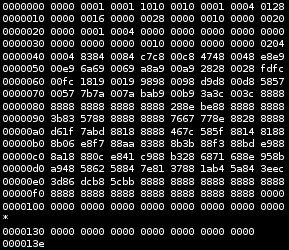
\includegraphics{img/machin-code.png}
    \caption{Example of machine code (Source: \href{https://bit.ly/3sQendj}{https://bit.ly/3sQendj})}
    \label{fig:machine_code}
\end{figure}

\subsection{Source code}
As shown above, machine code is very difficult to write by hand. So instead of writing machine code directly, programmers usually write codes with higher level programming languages that are closer to human language. Examples of them includes: C, C++, Java, Python, Javascript, php, C\#, Ruby, R, VisualBasic, etc. The code we wrote using higher level language are usually called \textbf{source code} (Fig.~\ref{fig:source_code_python}).
\begin{figure}[h]
    \centering
    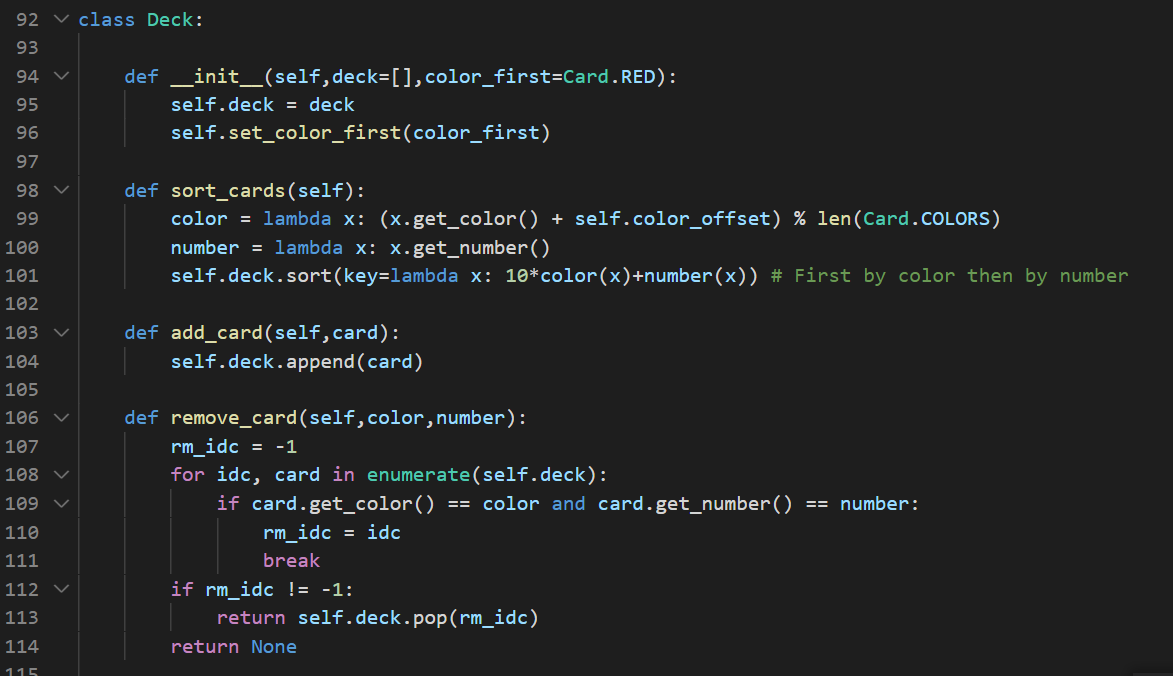
\includegraphics[width=0.6\textwidth]{img/python-code.PNG}
    \caption{Source code in Python (Source: me)}
    \label{fig:source_code_python}
\end{figure}

\subsection{Compiler}
Since computers understand only machine code but not our source code, we will need to convert source code to machine code through a program. This program is usually called a \textbf{compiler}. A compiler takes source code in high level language and compiles it into file called \textbf{executables} that contains machine language (Fig.~\ref{fig:compiler}). The executables (in Windows it has a file extension of .exe) can then be run by the computer.

\begin{figure}[h]
    \centering
    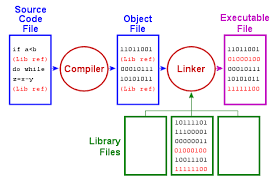
\includegraphics[width=0.6\textwidth]{img/compiling.png}
    \caption{Compiler compiles source code to machine code (Source: \href{https://bit.ly/3sQendj}{https://bit.ly/3sQendj})}
    \label{fig:compiler}
\end{figure}

\subsection{Interpreter}
Some languages, like Python, runs a bit differently. Instead of compiling the whole file from source code to executable, they compile source code line by line during run-time. The program responsible for this conversion is called an \textbf{interpreter} instead of a compiler.

\section{Epilogue: Mentality of coding}
In the rest of the semester, we will learn how to code! But before getting too hype about that, one should remember we are only teaching the \textit{essentials} of coding - Similar to how a guy who knows how to read the score doesn't necessarily knows how to compose music. 

Learning the basics of code will only equipe gives you basic skills of \textit{reading and writing} code. To \textit{create and express yourself}  with code, you will need much more than that. Not only would you need to \textit{practice} a lot, but you will also need to \textit{read and learn} a lot. That takes time and you should not feel ashame of not getting stuff as you go on. 

Furthermore, you are not alone! Always discuss with your friends whenever you don't understand something and share your thoughts and ideas through communication - three heads are better than one!

Finally, have fun coding!
\printbibliography
\end{document}


